\chapter{Implementation}
  The language of choice we used for the implementation is python2.7. Although we also could have implemented the extension in c/c++ since the basic version
  was already written in this language, python does have some key advantages we did not want to miss.
  \begin{description}
    \item [Rapid prototyping]
    Since our algorithms can easily work on a given set of data completely independent and the interfaces to get the data from are clearly defined and accessible,
    using a lightweight language like python had the benefit of not having to embed our new code into the existing environment. Although it still can be implemented 
    in the native language C/C++ for our scenario, this will take some more time and effort, which was not the focus of this work.
    \item[Existing libraries]
    like NetworkX in python made it particulary easy for us to map real world scenarios to graph abstractions as we did not have to create those structures ourselves.
    Although there are some libraries that provide graph abstractions in C/C++ we could not have as easily employed them due to their copyright restrictions and 
    the closed source virtue of our target system.
    \item[Faster Debugging]
    Especially the initial phase of the project was errorprone and needed a lot of debugging. Not having to recompile after every fix turned out to be
    a great saving of time. Not to mention the live debugging capabilities of python, which was really helpful.
    \item[Existing APIs]
    Fortunately also the code for interaction with the interfaces (SNMP/SSH/Telnet) of the WLC was written in Python, so we could easily 
    integrate it into ours and had no problem gathering the 'seen'-data. Unfortunately for you those libraries are closed source to the public.
    \item[Maintainability]
    As python has the reputation of being an easy to learn language, this was another benefit and played absolutely in our favor with the goal of
    keeping the code simple, lightweight and reuseable by someone else.
  \end{description}
  \begin{figure}[t]
    \centering
    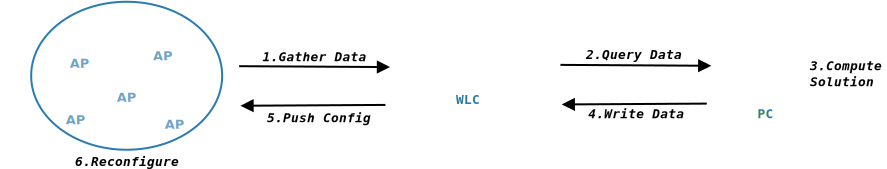
\includegraphics[width=1\columnwidth]{figures/dataflow}
    \caption{General flow of information for our scenario}
    \label{fig:dataflow}
  \end{figure}
\section{Dependencies}
  As already mentioned we used NetworkX\cite{hagberg-2008-exploring} to model our graphs and work with its elements.
  NetworkX's rich features like ``has\_path'' made things especially easy in computing the survival paths.
  Another library we used is python collections. \cite{python_collections}
  This library implements specialized container datatypes additionally to those shipped with standard python.
  It's `Counter` structure is used to create the channel-lists and retrieve the most or least used elements.
  We extended this library for our convencience since it did only provide the functionality for getting the most common element from its list and not the least common,
  which we needed. \footnote{It is worth mentioning that the request for including this method was already issued at 01/2013 http://bugs.python.org/issue16994}
  The only closed source library we used is the herein before mentioned library to query the WLC for the data of the APs. Nevertheless gathering the data can also
  easily be separated and outsourced to different interfaces.
\section{Structure of the Code}
  We split the code in two modules:
  \subsection{Interfacing Outer World and Managing Data}
  The name of the module is wlc_com. This module's responsibilites are:
  \begin{description}
   \item[Receiving the necessary data]
    For this purpose we use the closed source python library 'testcore', which creates a SSH/Telnet connection to the WLC and parses its tabledata.
    The information we receive is of the following form:
    \begin{table}[p]
      \begin{tabular}{clll}
	Device Mac Address & Module Mac Address & Seen Module Mac Address & \ac{SNR}\\ \hline
	ece55574a4d5 & ece555ffd61e & ece555ffd5bf & 56 \\
	ece55574a4d5 & ece555ffd6cc & ece555ffd5b9 & 48 \\
	ece55574a4a5 & ece555ffd667 & ece555ffd5d6 & 33 \\
	... & ... & ... & ...
      \end{tabular}
      \caption{Mesh network topology representation in table format on a lancom WLC. Device mac address is the LAN mac address, the module mac address is
      the address of the module which is equipped on the device and which receives the Beacons with the ESSIDs of other modules, which in turn translates
      the ESSID to the mac address of the opposing module. The \ac{SNR} describes thereon the quality of the link between those two modules.}
     \end{table}
    
    \item [Transform the data to a networkX graph]
      The tabledata from above can then be molded into a directed, weighted networkX graph. Where we create a node for each mac address and module mac address and attach a boolean
      attribute to it to tell them apart. 
      In parallel we add two types of edges:
    
      \begin{itemize}
	\item Fake edges between module-nodes and device-nodes with an attribute "SNR" which contains the maximum possible value for this attribute.
	
	\item Real edges for each line in the table above, where the two nodes are the module mac address pairs. 
	  Note that one row in the table represents just a directed edge from one module to the other. We only respect two-sided connections,
	  since one-sided edges are mostly of poor quality and would further complicate finding a solution.
	  As we have two SNR-values for a single undirected edge when merging two directed edges, we are at liberty to chose.
	  Currently we are using the average of both values, but implemented an option to use the larger or the smaller value if favoured.
	  Especially the lower SNR value might better represent a connection for more pessimistic scenarios.
      \end{itemize}
    
    \item[Conducting a validity check on the result]
      Before generating the configuration and sending the result to the WLC we have the option perform some sanity checks on the outcome.
      Among others we test for the following:
	\begin{description}
	 \item [Connectedness of the graph]
	  Is each device connected to the network, or are there disconnected components?
	 \item [Channel / Band conformance]
	  Do modules which are supposed to establish a connection use the same channel and Band?
	 \item [Using allowed channels]
	  Are only channels used which have been specified as input?
	 \item [Device Module separation]
	  Are all devices only connected to their modules over module-device edges?
	\end{description}
    \item [Send results back to the WLC]
      If we were able to compute a solution and all checks passed we again establish a connection to the WLC and write back a network topology and channel assignment
      configuration. This configuration will then be enforced on the accesspoints by the managing WLC.
      This is done by configuring each module to use only the assigned channel and set entries in the network topology table. Depending on other parameters the
      accesspoints will then after a while receive their specific configurations and act on those.
  \end{description}
  
  \subsection{Work on the Graphs} Working on NetworkX Graphs to find the desired solution
    As we need the data in a format we can work with, we thereon transform it to a networkX graph. 
    Therefore we create a weighted undirected networkX graph from the given directed weighted graph and take the 
  

  Kann man den Code in gruppen einteilen, wenn ja in welche? Welche Funktionen gibt es? Was tun diese?
  \subsection{Selecting the Network Topology}
    \subsubsection{Minimal Spanning Tree}
    \subsubsection{Adding Redundand Paths}
  \subsection{Coloring the Edges/Modules}
  \subsection{Validating the Result}
    Checking the coloring and channel assignment after the algo run
\section{Problems}
  \begin{description}
   \item[Have there been problems with the implementation?]
   extracting data from strangly ordered tables of lancom devices was tricky
   \item[What else could count as a problem / What else could fit in here?]
  \end{description}
\section{Run It Yourself}
  \begin{description}
   \item[What is needed to run the algorithm on your own machine?]
    Input data is required (aka which access point sees what other acces point with what Signal to Noise Ratio?) \newline
  \end{description}
